
\subsection{Related Work}
There is growing evidence that demand-side resources (DSRs) can participate in ancillary services, thus substituting the need for traditional ancillary service resources. However, the DSRs that can provide ancillary services vary greatly in composition, and have distinct properties. Most of the research on DSRs to provide transmission-level services has focused on specific services using a particular set of loads connected to the grid. This is partly due to varying characteristics of DSRs and partly to the suitable control architecture for the proposed services. 

A common set of resources studied in connection to DR are thermostatically controlled loads~\cite{Molina_Garcia_2011,Kara_2012,thavlov2014utilization,mathieu2012using}, such as electric space heating \cite{mathieu2012using,thavlov2014utilization}, residential and industrial refrigeration \cite{lakshmanan2014energy}, and space heating using heat pumps \cite{halvgaard2012economic}. Thermostatically controlled loads are valued for their ability to provide ancillary services because of the inherent thermal inertia present in the systems. The thermal inertia acts as energy storage, permitting the curtailment or deferral of power consumption. The application of TCLs as a DR mechanism can also be seen in industrial settings such as large refrigeration systems \cite{rahnama2013integration}, the heating of bitumen tanks \cite{cheng2014availability}, and indoor climate control using HVAC \cite{blum2013ancillary}. 

Batteries can also provide ancillary services through demand response. Electric vehicles (EVs) can be considered as mobile batteries with additional time varying constraints. By changing their charge patterns while guaranteeing the mobility needs of the owner, EVs can offer the demand-side flexibility needed to provide ancillary services to the grid \cite{zarogiannis2014dynamic,kara2015estimating}. 

The potential of using the dimming of lighting in office buildings for DR is presented in \cite{rubinstein2011demand}. A pilot project in Denmark also used the lighting system in an industrial green house for DR, showing the potential of using DR to manage congestion in the distribution system. 

Water pumps--used in wastewater treatment systems and agriculture--are also considered a promising resource for ancillary services. Specifically, in \cite{halvgaard2014waste}, the authors suggest that water can be temporarily stored in pipes and tanks, hence delaying the transportation for treatment in waste water treatment systems. The load flexibility of agricultural water pumps stems from the inherent flexibility in the time of irrigation.
%The response of the pumps is fast, and depending on the system state and weather conditions can be sustained from medium to long time. The system requires a certain amount of energy to move the water around, and is therefore deferrable. Due to the pumps there may be constraints on the cycling.
%Furthermore, 50\% of the energy consumption of a waste water treatment plant is spent on the aeration process, which can also be deferred. 

In this paper, we examine the use of DR when system reliability is jeopardized. A great deal of research has focused on DSR-specific controller design and limitations due to load characteristics and comfort needs. Specifically, many aggregation frameworks exist in the literature that overcome cycling constraints and response frequency limitations. Hence, instead of focusing on the design of such DSR-specific controllers, we assume that AS provided by DSRs will be sold to system operators by an aggregator, and that the aggregator is responsible for control accuracy. 
Our objective in this paper is to discuss and formulate ideal performance requirements for ancillary services in a number of relevant features, and to provide a market clearing mechanism that selects a portfolio of resources in a resource-agnostic and performance-oriented way. By doing so, we propose a strategy in which (i) we remove the barriers preventing unconventional resources from participating in AS markets due to the static nature of AS market definitions and requirements, and (ii) we provide a fair and performance-based market clearing structure in which the unused potential of DSRs can be easily incorporated.

\subsection{Properties}
The identified DSR parameters are given as follows:
%\kara{I think here we need a discussion of parameters that we are using in Section 4 to define $\kappa$} \kara{I think the properties should be of aggregations, not necessarily the DR resources}
%\olge{I know I probably spend way too much time looking at microcontroller timing diagrams, but would it help trying to put all the parameters into a single timeline drawing like the sketch in figure {\ref{fig:resourcecharacteristics}} ?}
%\begin{figure}[htb!]
%\centering
%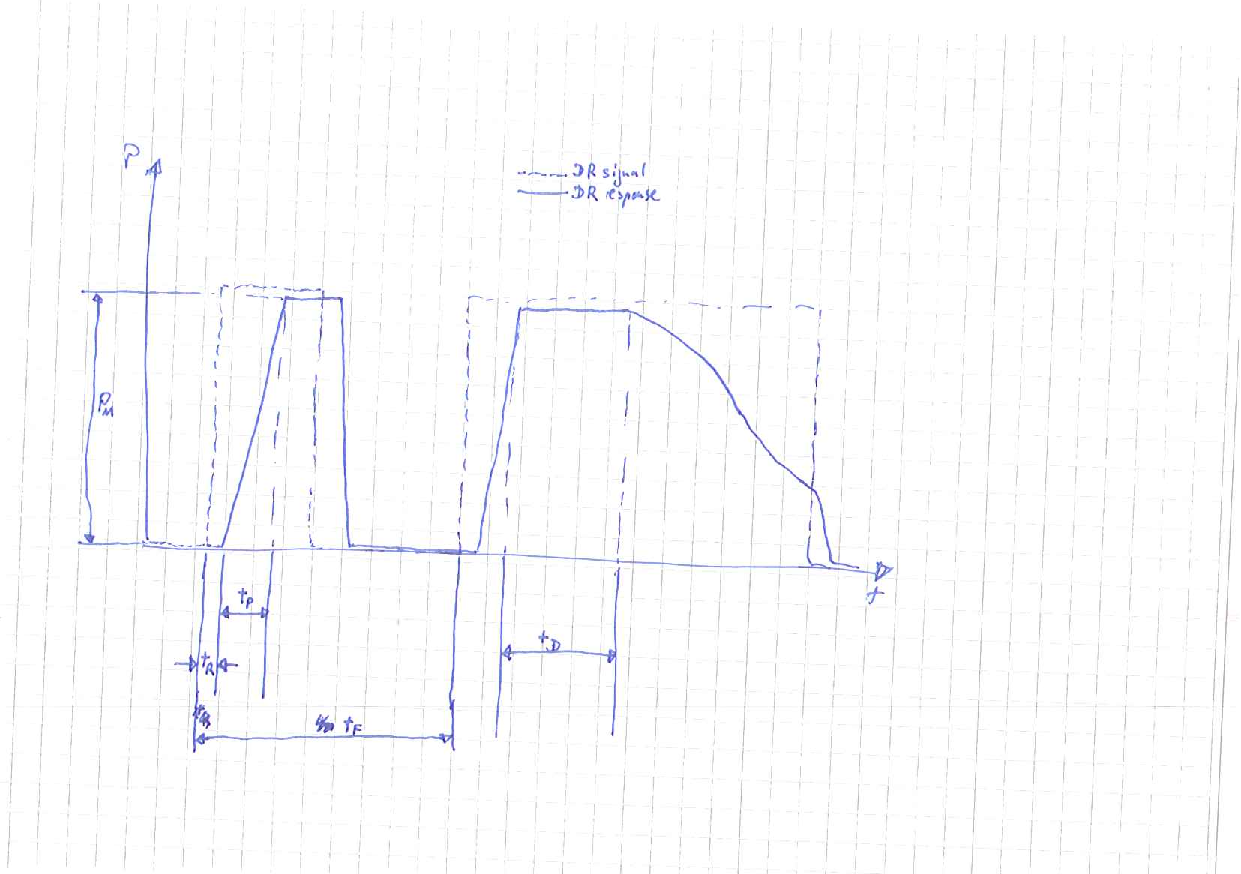
\includegraphics[width=1\columnwidth]{20150731150249153.pdf}
%\caption{Characteristics of demand side resource [sketch].}
%\label{fig:resourcecharacteristics}
%\end{figure}

\begin{description}
    \item[Response time] This is the time it,takes for a unit to receive a DR signal and react upon it. %\textcolor{red}{I'm not sure on this one, since pretty much all of them have fast response time, depending on the control architecture and the communication system, which are not inherent to the DER}
    \item[Response duration] How long is a pool of these units able to sustain service provision: short, medium or long. %\textcolor{red}{Again, this is a tough one, since this will depend on the state of the portfolio/unit}
    \item[Response magnitude] This the \emph{amount} of load used by the DR resources that can be increased or decreased. The increase capability is defined as the \emph{take} magnitude and the decrease capability is defined as the \emph{shed} magnitude.
\end{description}


\subsection{Unused Potential of DSRs and Barriers to DSR Participation}

\label{subsec:unused}
Although DSRs provide additional freedom to help shape response compared to traditional AS providers, the existing ancillary service market rules and requirements are a strong barrier to DSR market participation. A recent study identifies such barriers in the US\cite{cappers2013assessment}. The rules and requirements that limit resource participation in different markets are not consistent among different RTOs and ISOs; however, the authors identify three major groups of these rules: rules on the size of the resource, rules on the measurement and telemetry of the resource, and rules on market bidding time. Out of six different ISOs and RTOs in the US, only one allows load aggregations to provide regulation services, and only two allow aggregation participation as a spinning reserve provider. Furthermore, only two ISOs and RTOs allow aggregate telemetry. Providing telemetry at an individual resource level increases the overall cost of metering, making it challenging for DSRs to provide cost-competitive AS. Finally, most of the AS markets procure in day-ahead markets, and day-ahead DSR participation is harder due to increasing uncertainty in DSR flexibility forecasts.  

In order to accommodate the slow-ramping resources as well as DSRs in the AS markets, there is an increasing need to either split AS into different service classes or parametrize the service definition so that the resources are selected only by their ability to satisfy the system needs. The ideal resource to satisfy the system need is one with ``unlimited capabilities in terms of response time, energy output, ability to frequently reverse their output, ability to respond and follow the AGC setpoint changes, and size.''\cite{makarov2008assessing}\footnote{For this kind of response to be optimal, changes must be made to the AGC algorithm \cite{peydayesh2012effects}.} To include and incentivize the participation of technologies that in some parameters are closer to the ideal than those defined by the current service and market requirements, two methods can be utilized: product differentiation and product restructuring.

Some transmission system operators, like PJM, have already suggested that better service performance is more valuable than simply adhering to traditional rules and requirements, and split their regulation market into a slow service product and a fast service product. 
This work explores the alternative: restructuring the market so that all technologies can participate in the same market, and the system operator can optimize the use of the resources based upon their capabilities. This entails reformulating the temporal and market requirements, and removing the requirements that implicitly assume that the services are provided by traditional generators, thus making the requirements technology-agnostic. %In the next section, we discuss the \emph{new proposition}.\kara{to be filled} 


 